\documentclass{report}
\usepackage{graphicx}
\usepackage{enumitem}
\usepackage[margin=1.5cm]{geometry}

\title{\Huge \textbf{Use Cases}\\ \Large Arfib}
\author{
    Henrique Romão \\ up202108067@up.pt
    \and
    Mariana Bessa \\ up202107946@up.pt
}

\begin{document}

\maketitle

\tableofcontents

\chapter{System Requirements}

\newpage
\chapter{Use Case Diagram}

\begin{figure}[ht]
    \centering
    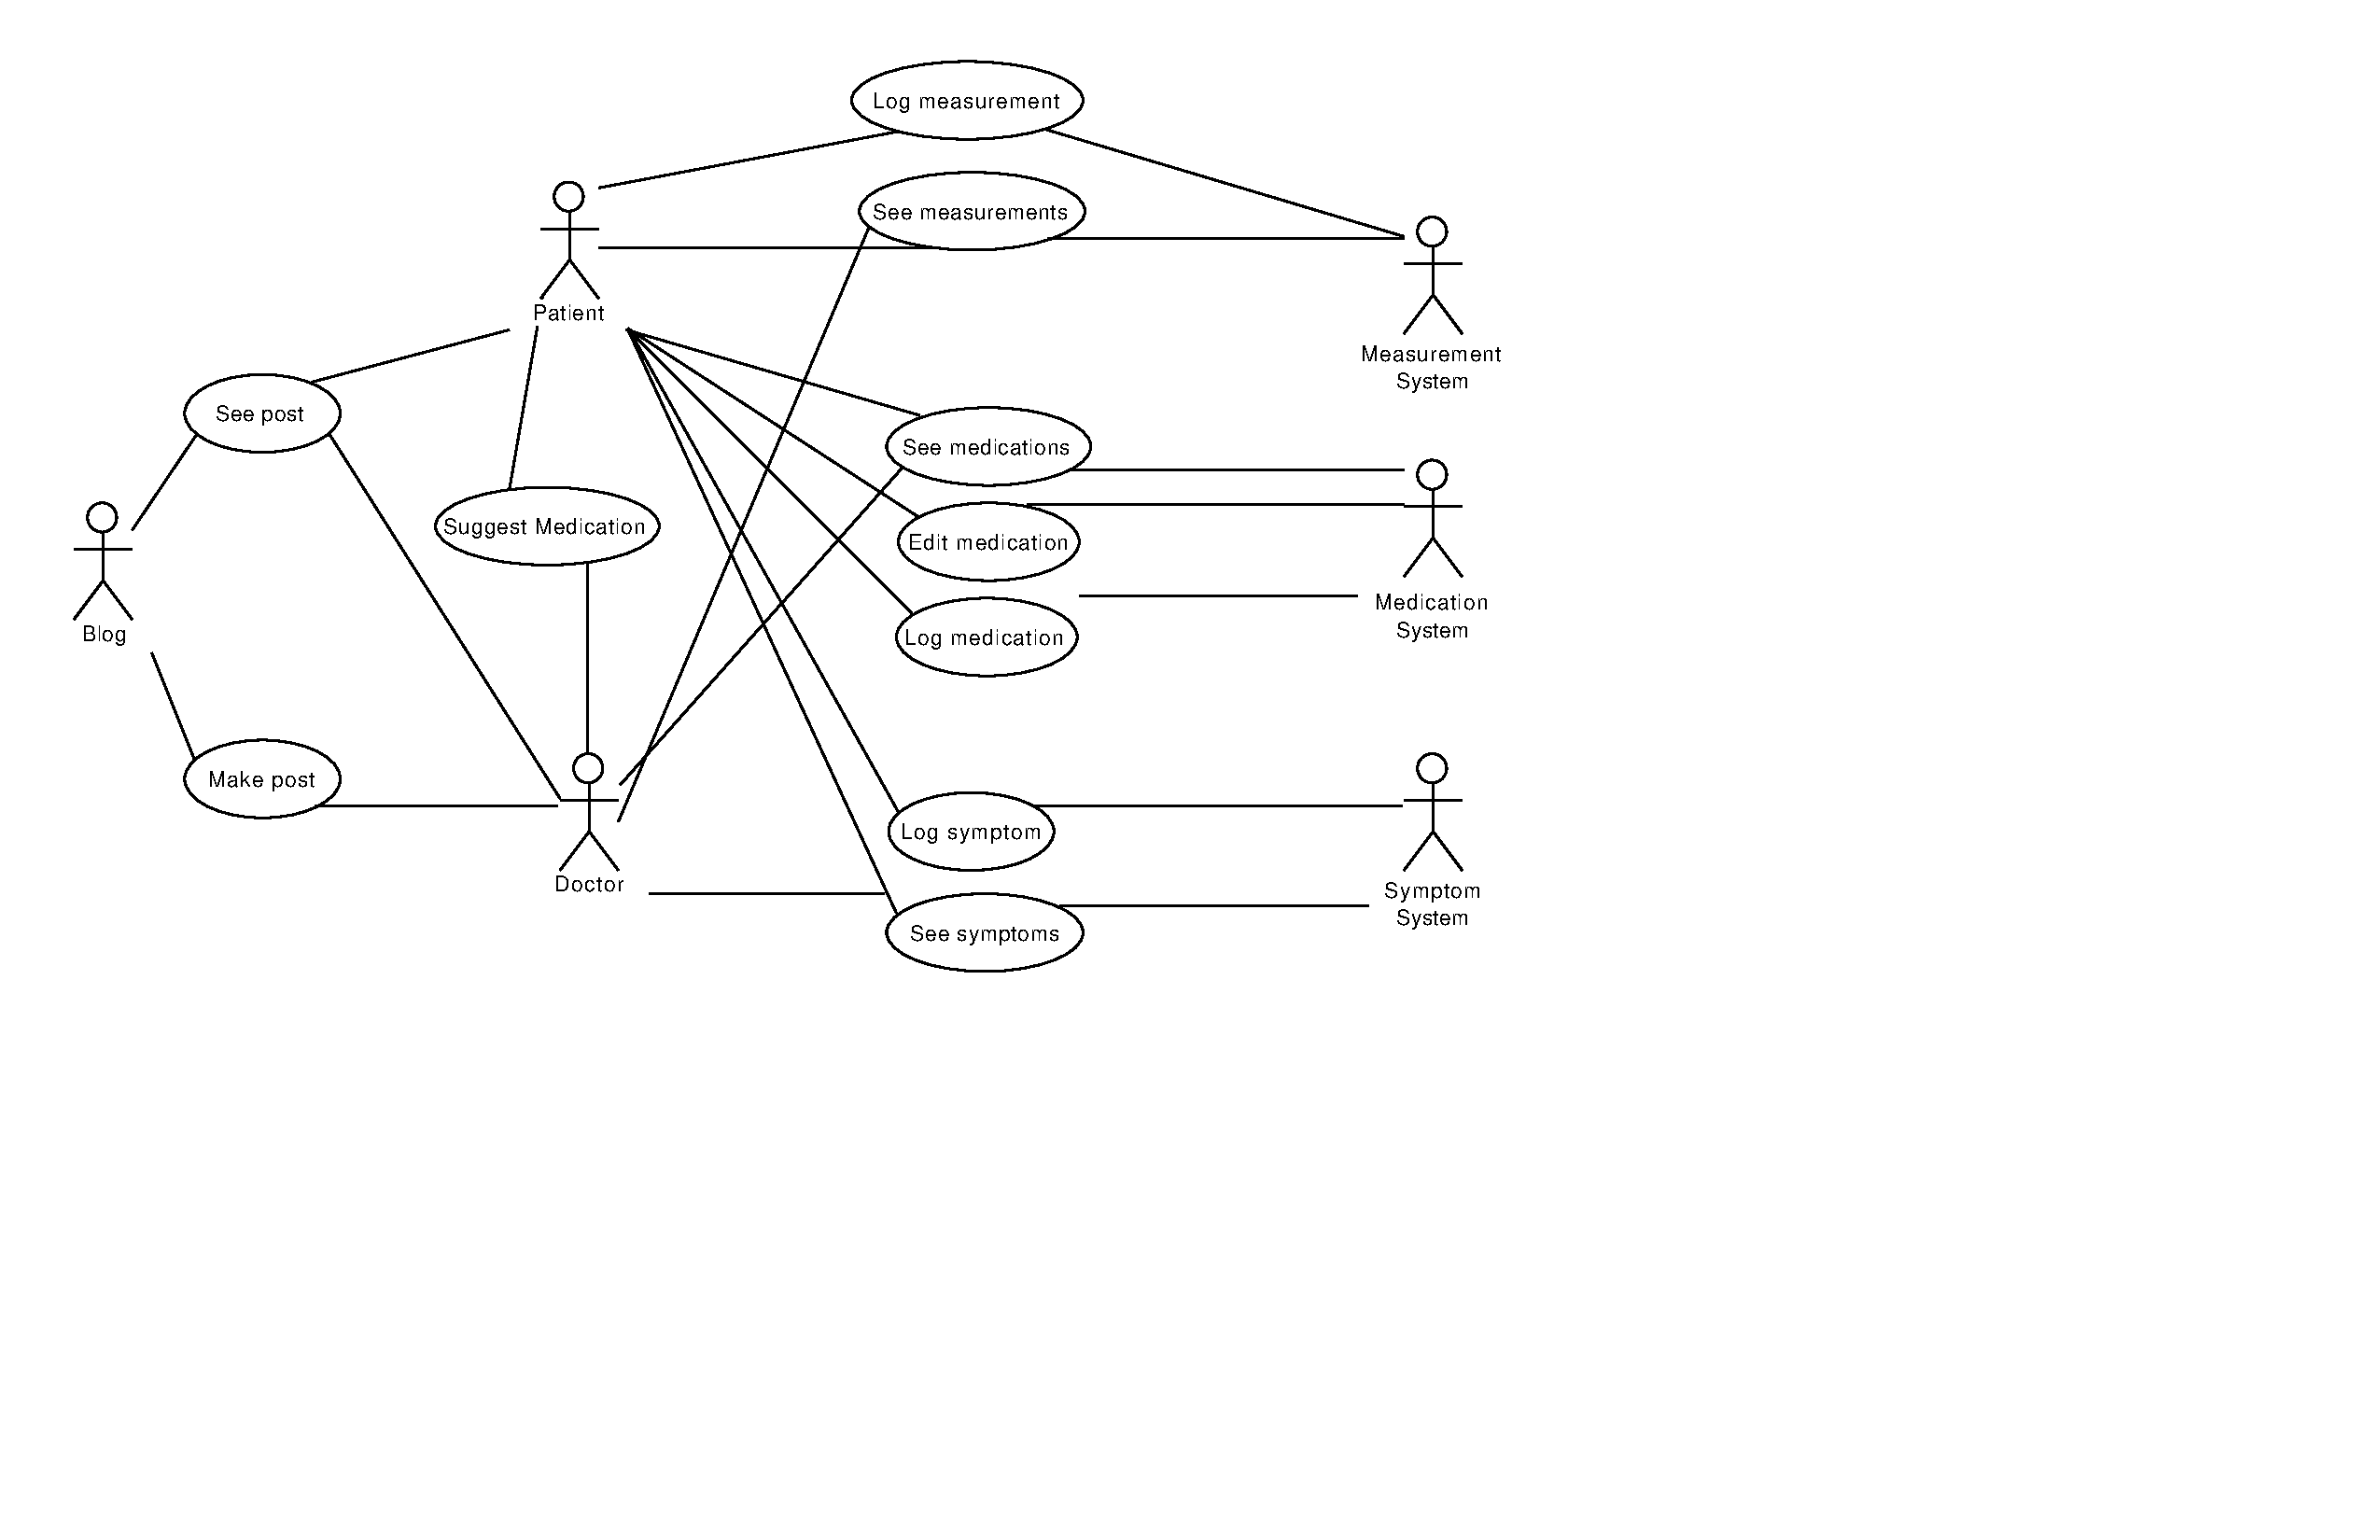
\includegraphics[width=\linewidth]{General Use Case Diagram.pdf}
    \caption{Use Case Diagram.}
    \label{fig:Use Case}
\end{figure}

\chapter{Use Case Description}
\section{Measurement}
\subsection{Log Measurement}
\begin{figure}[ht]
    \centering
    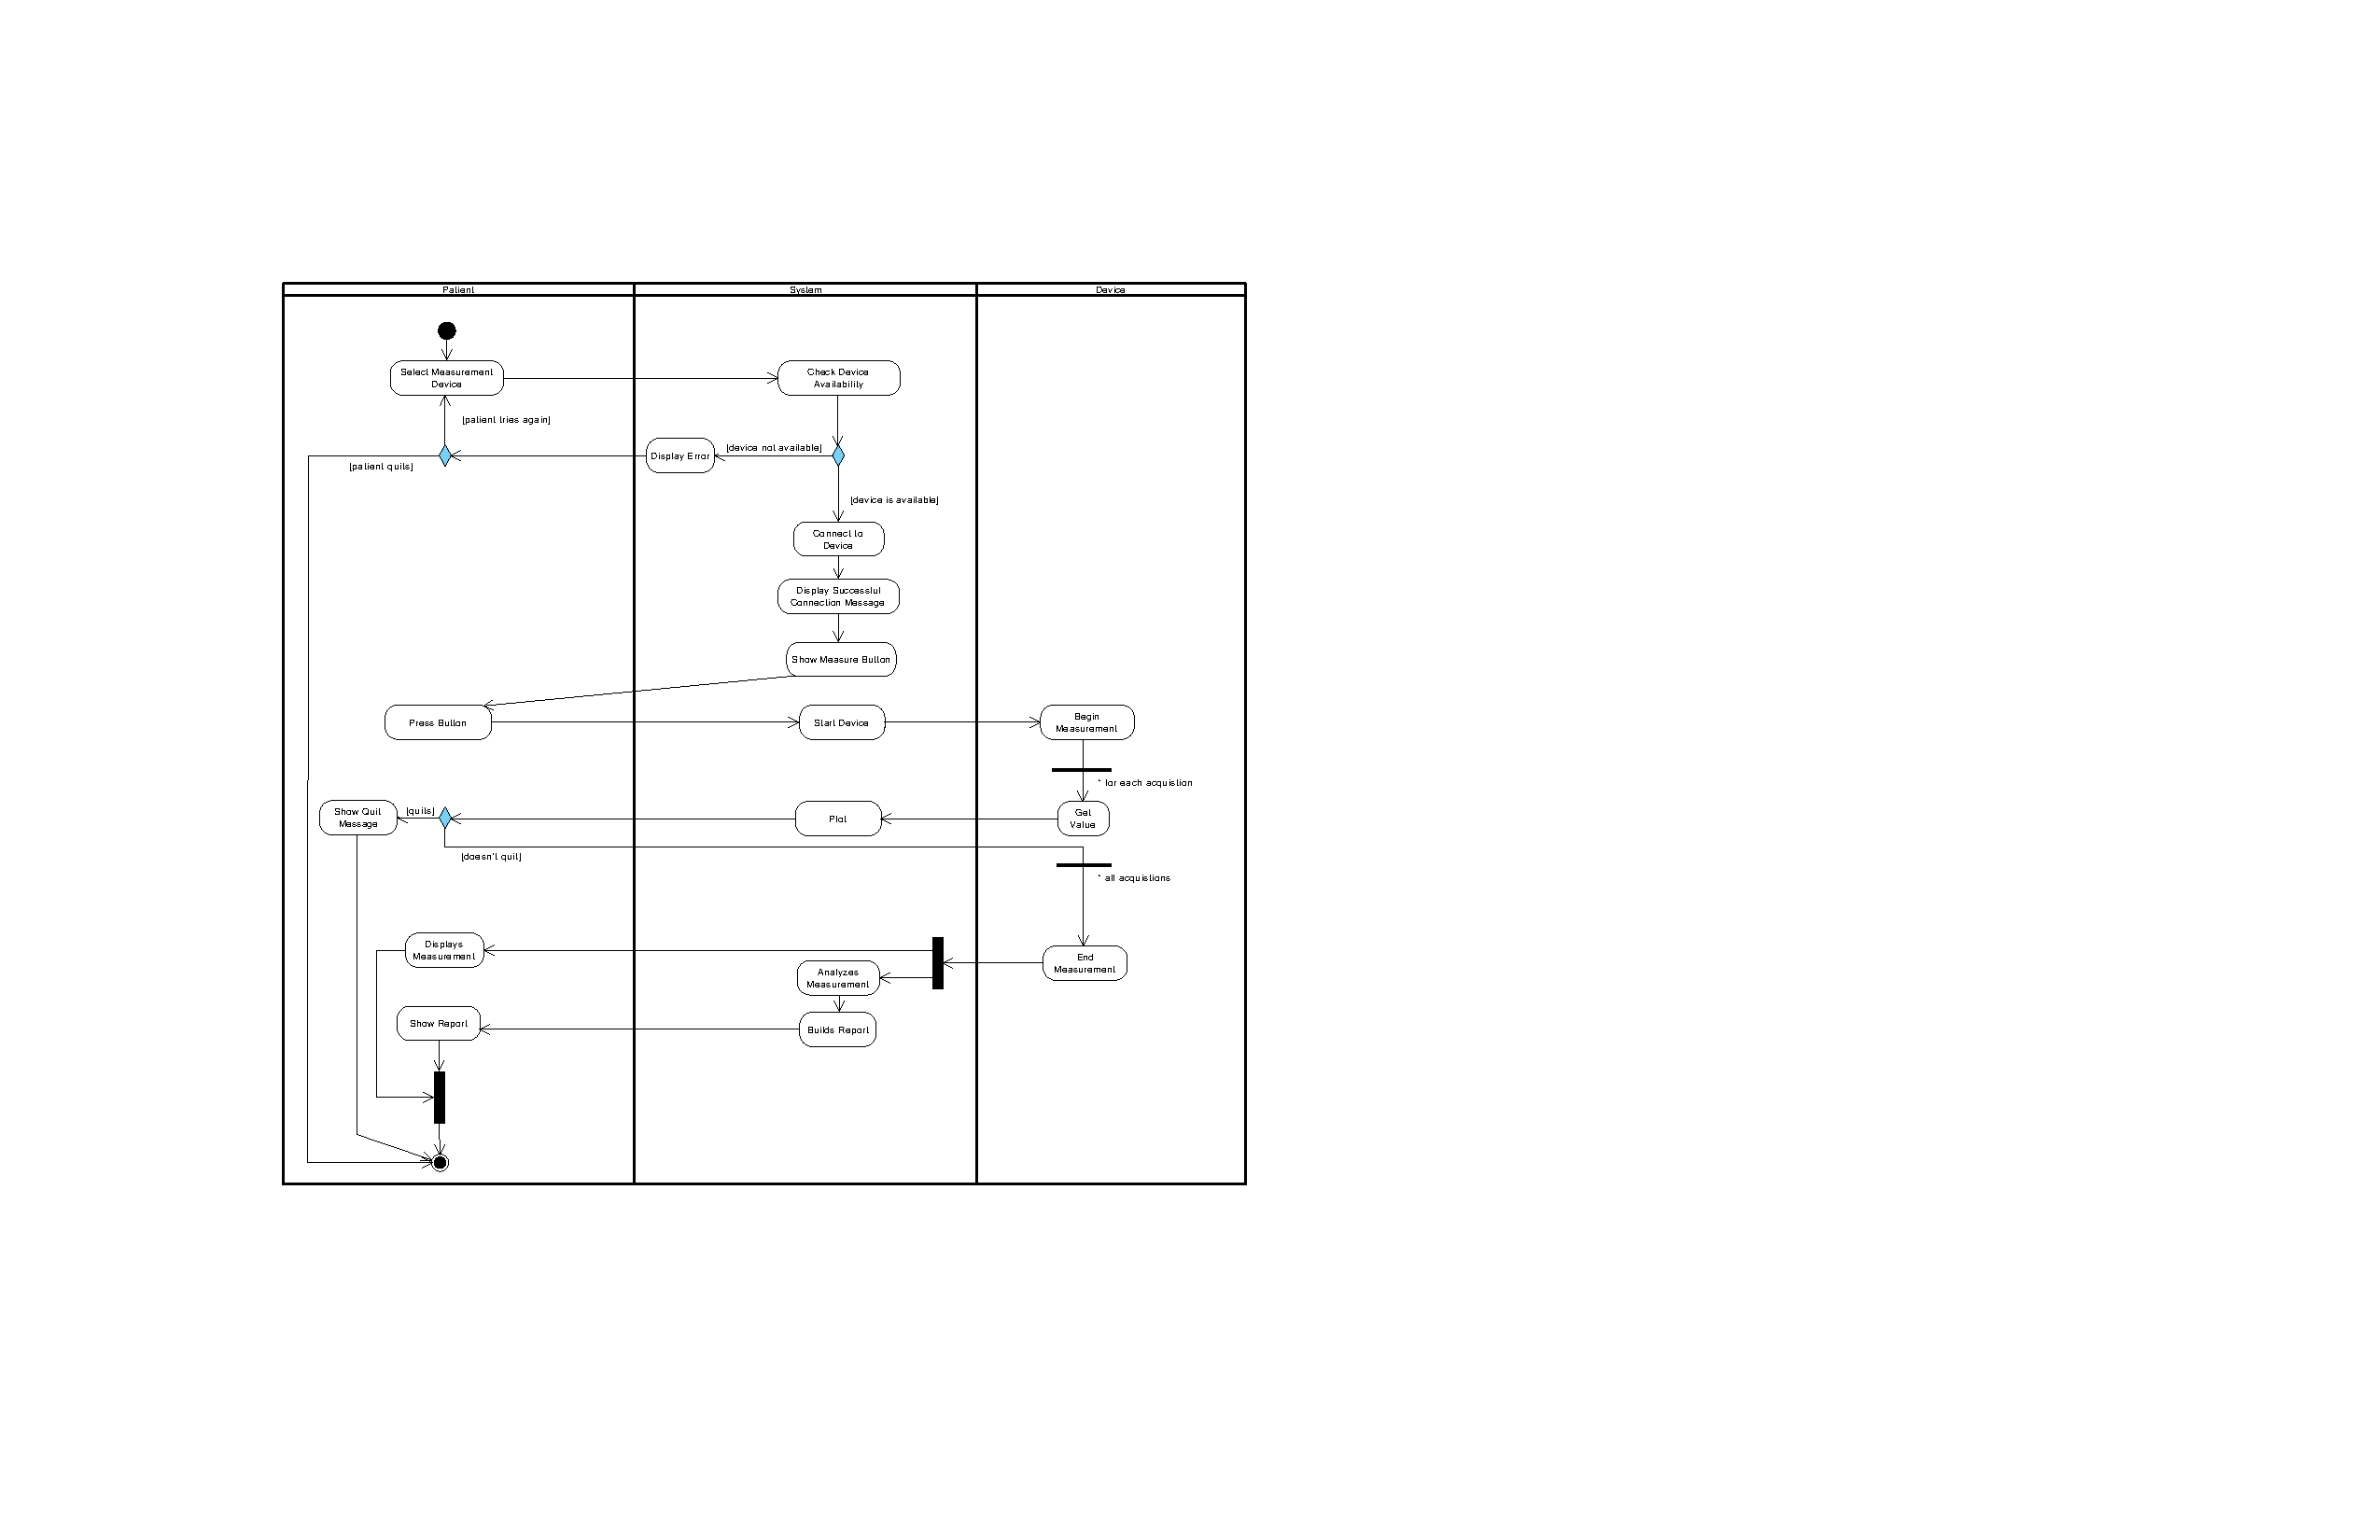
\includegraphics[width=0.75\linewidth]{Log Measurement.pdf}
    \caption{Log Measurment Activity Diagram.}
    \label{fig:Log Measure}
\end{figure}


\subsection{See Measurement}
\subsubsection{Brief Description}
This use case allows a patient see its own previous measurements, or allows a doctor to see the previous measurements of their patients.
Both have access to a list of the measurments, allowing them to choose a specific one to see in more detail.

\subsubsection{Step-by-Step Outline}
\paragraph{Basic Flow}
\begin{enumerate}
    \item Select patient's measurements page.
    \item Check access.
    \item Display previous measurements.
    \item Choose measurement of interest.
    \item Display full information about measurement of interest.
\end{enumerate}

\paragraph{Alternative Flows}
\begin{enumerate}[label=A\arabic*.]
    \item Doctor or patient does not have access.
    \item Show error message.
    \item Quit.
    \item See measurement closed.
\end{enumerate}

\section{Medications}
\subsection{Log Medication}
\subsection{See Medications}
\subsection{Edit Medication}
\subsection{Suggest Medication}

\section{Symptoms}
\subsection{Log Symptom}
\subsection{See Symptoms}

\section{Blog}
\subsection{See Post}
\subsection{Publish Post}

\end{document}